\section{Experimental Evaluation}
\label{sec:result}

To demonstrate the ability of resource monitoring and control in the Charon framework, we designed a simple experiment in which a single computing cluster runs the scientific AI application~\cite{babu2022deep} to process live streaming data from a beamline detector. In this experiment, the rate at which the AI model processes X-ray images should ideally be matched with the data generation rate of the detector in order to prevent any data loss. The controller in this experiment is responsible for keeping up with the data generation rate by controlling the number of application instances, which changes the global data processing rate.

\subsection{Setup}

We use the Chameleon~\cite{chameleon} testbed to set up a single-node cluster and provision it using the proposed framework. The provisioning installs tools to bring up Nvidia's GPU support and container run time. At the end of provisioning, the cluster is ready to accept user applications while monitoring their resource usage in real time. Additional tooling and visualization can expose the performance information to users, including Graphana dashboards using the data monitored by NRM and sent to a Prometheus instance.

The application workflow is as follows.

\begin{itemize}
\item{\textbf{Data generator}} loads the recorded scientific data of a beamline detector and streams the data as individual frames at the desired rate of 1,000 Hz.
\item{\textbf{Distribution server}} takes the stream and distributes frames to any connected consumer instance; the distribution follows a simple round-robin policy among all connected consumers, to balance the load. 
\item{\textbf{Consumer} runs the PtychoNN AI model to process frames; output data frames go to the next stage for aggregation.}
\end{itemize}

This workflow is implemented by using PvaPy, a Python data streaming infrastructure developed by the Argonne APS staff for use with some of their detectors, and mimics a real deployment. Additionally, we instrument the AI@Edge application, that is, the consumer in the workflow, to constantly publish application performance metrics through NRM. The Charon controller then communicates with NRM to analyze incoming metrics and make control decisions. One of the metrics we use in this control experiment is the number of queued frames (received by a consumer but not yet processed), indicating whether the application is behind the data generation rate. An increase in this metric means that the workflow cannot process data frames at the rate of data generation and needs more computing power.

\begin{figure}[!tb]
  \centering
  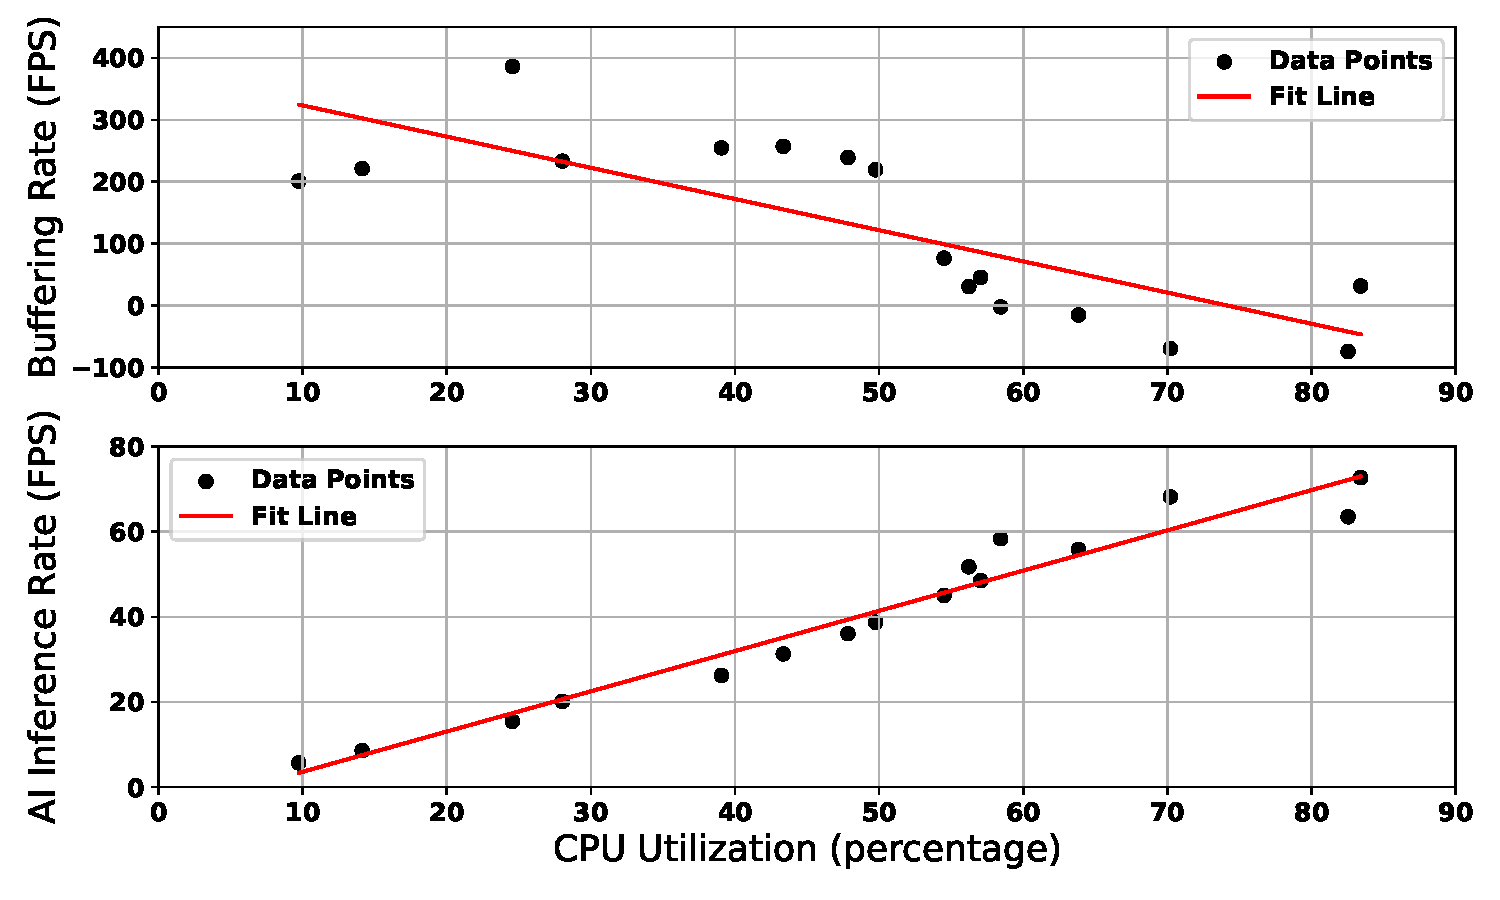
\includegraphics[width=\linewidth]{figures/linearity.pdf}
  \caption{Checking the linearity of the controlled variables.}
  \label{fig:linearity}
\end{figure}

\begin{figure}[!tb]
  \centering
  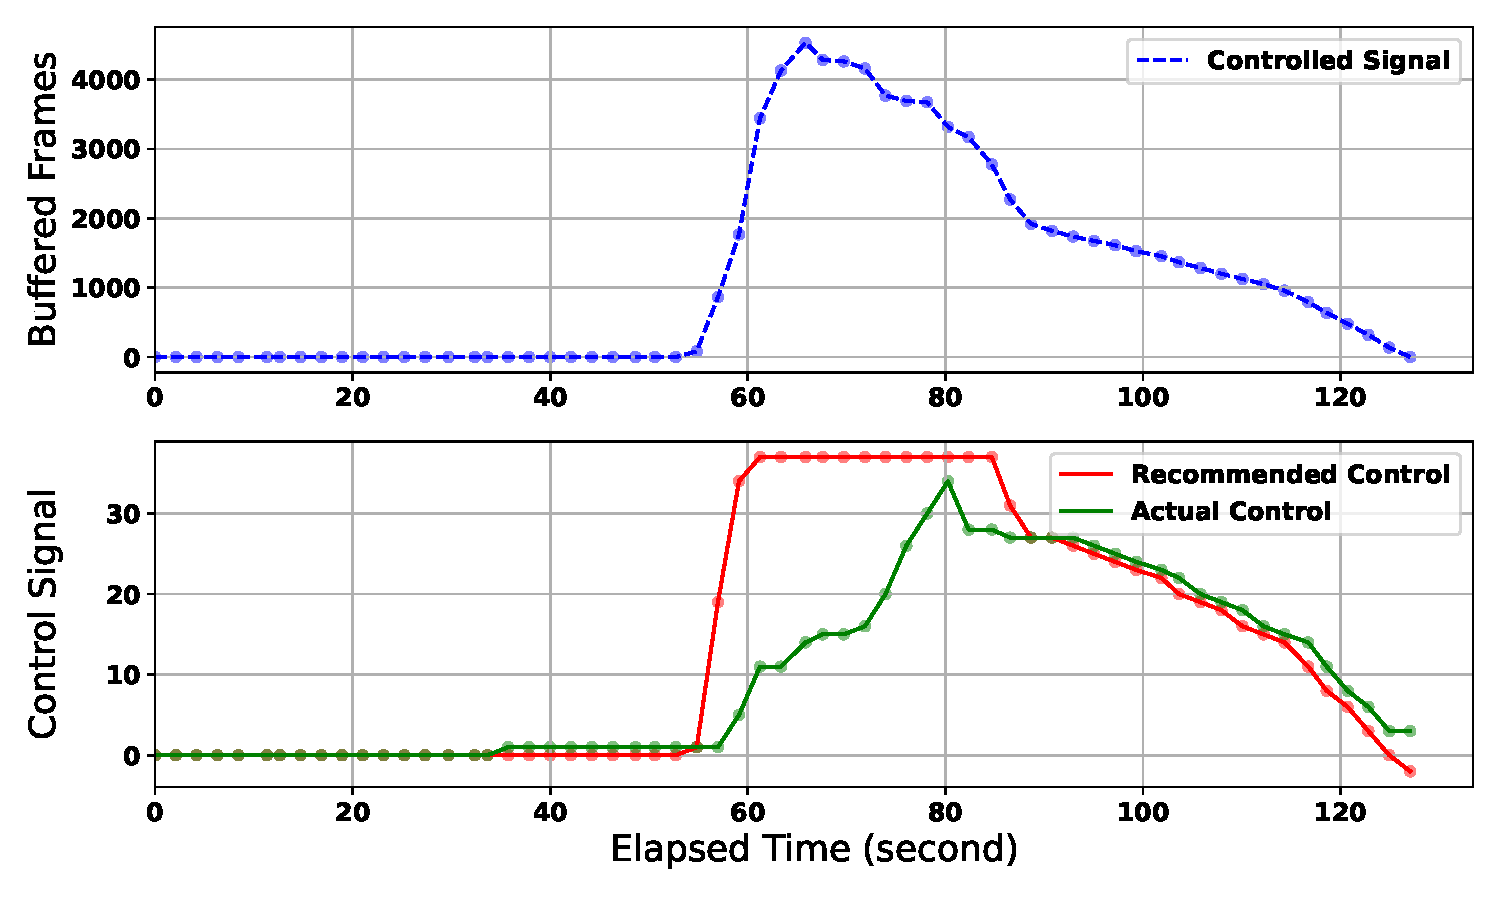
\includegraphics[width=\linewidth]{figures/control_result.pdf}
  \caption{Controlling to reduce frame buffering toward zero. $K_p = 1$ and $K_d = 3$ were used. The control signal is emitted to Kubernetes to modify the number of AI@Edge instances (consumers) at run time.}
  \label{fig:control-result}
\end{figure}

\subsection{AI Inference Management and Control}
\label{subsec:first-experiment}

First, we evaluate the impact of our controlled resources on overall performance. Since preprocessing of images is currently implemented as a sequential algorithm on the CPU, we consider preprocessing instances (containers) and CPU utilization to be the same metric (utilization between 0 and 100 is rate limiting for one container, between 100 and 200 for two containers, and so on). Note that we did not control the GPU resource because GPU resource division per application instance was unavailable outside of Nvidia's multi-instance GPU  technology~\cite{li2022characterizing}, which cannot be reconfigured dynamically. Nevertheless, this evaluation is part of the typical characterization process for the design of a controller. Figure~\ref{fig:linearity} displays the relationship between inference rate, buffering rate of the data, and CPU utilization. As we allocate more CPU resources, the buffering decreases while the AI inference rate increases. Therefore, we confirm that linearity in the relationship exists, enabling us to design a PID controller.

Given this characterization, we design a proportional-derivative controller, using the number of frames waiting for processing (queue length) as the signal to minimize. The following equation defines our controller:  $u(t) = K_p e(t) + K_d \frac{\delta e(t)}{\delta t}$, where $u(t)$ represents the control at time $t$, which is a proxy for CPU utilization at time $t$; $K_p$ is the proportional gain; $K_d$ is the derivative gain; and $e(t)$ is the error between the actual and desired queue values at time $t$. Figure~\ref{fig:control-result} illustrates how such a controller behaves on an experiment where the frame rate of the data generator is set to 1,000 frames per second. The controller waits an initial 20 seconds before starting, upon which new preprocessing containers are launched to respond to the growing queue length. Overall, around 30 container instances are progressively launched to handle the incoming frames. This controller design can be adapted further depending on needs; adjusting the control parameters $K_p$ and $K_d$ will change the aggressiveness of the control, leading to faster convergence but possible oscillation in the control.

\subsection{Adaptive Control Using Different AI Models}

\begin{figure}[!tb]
  \centering
  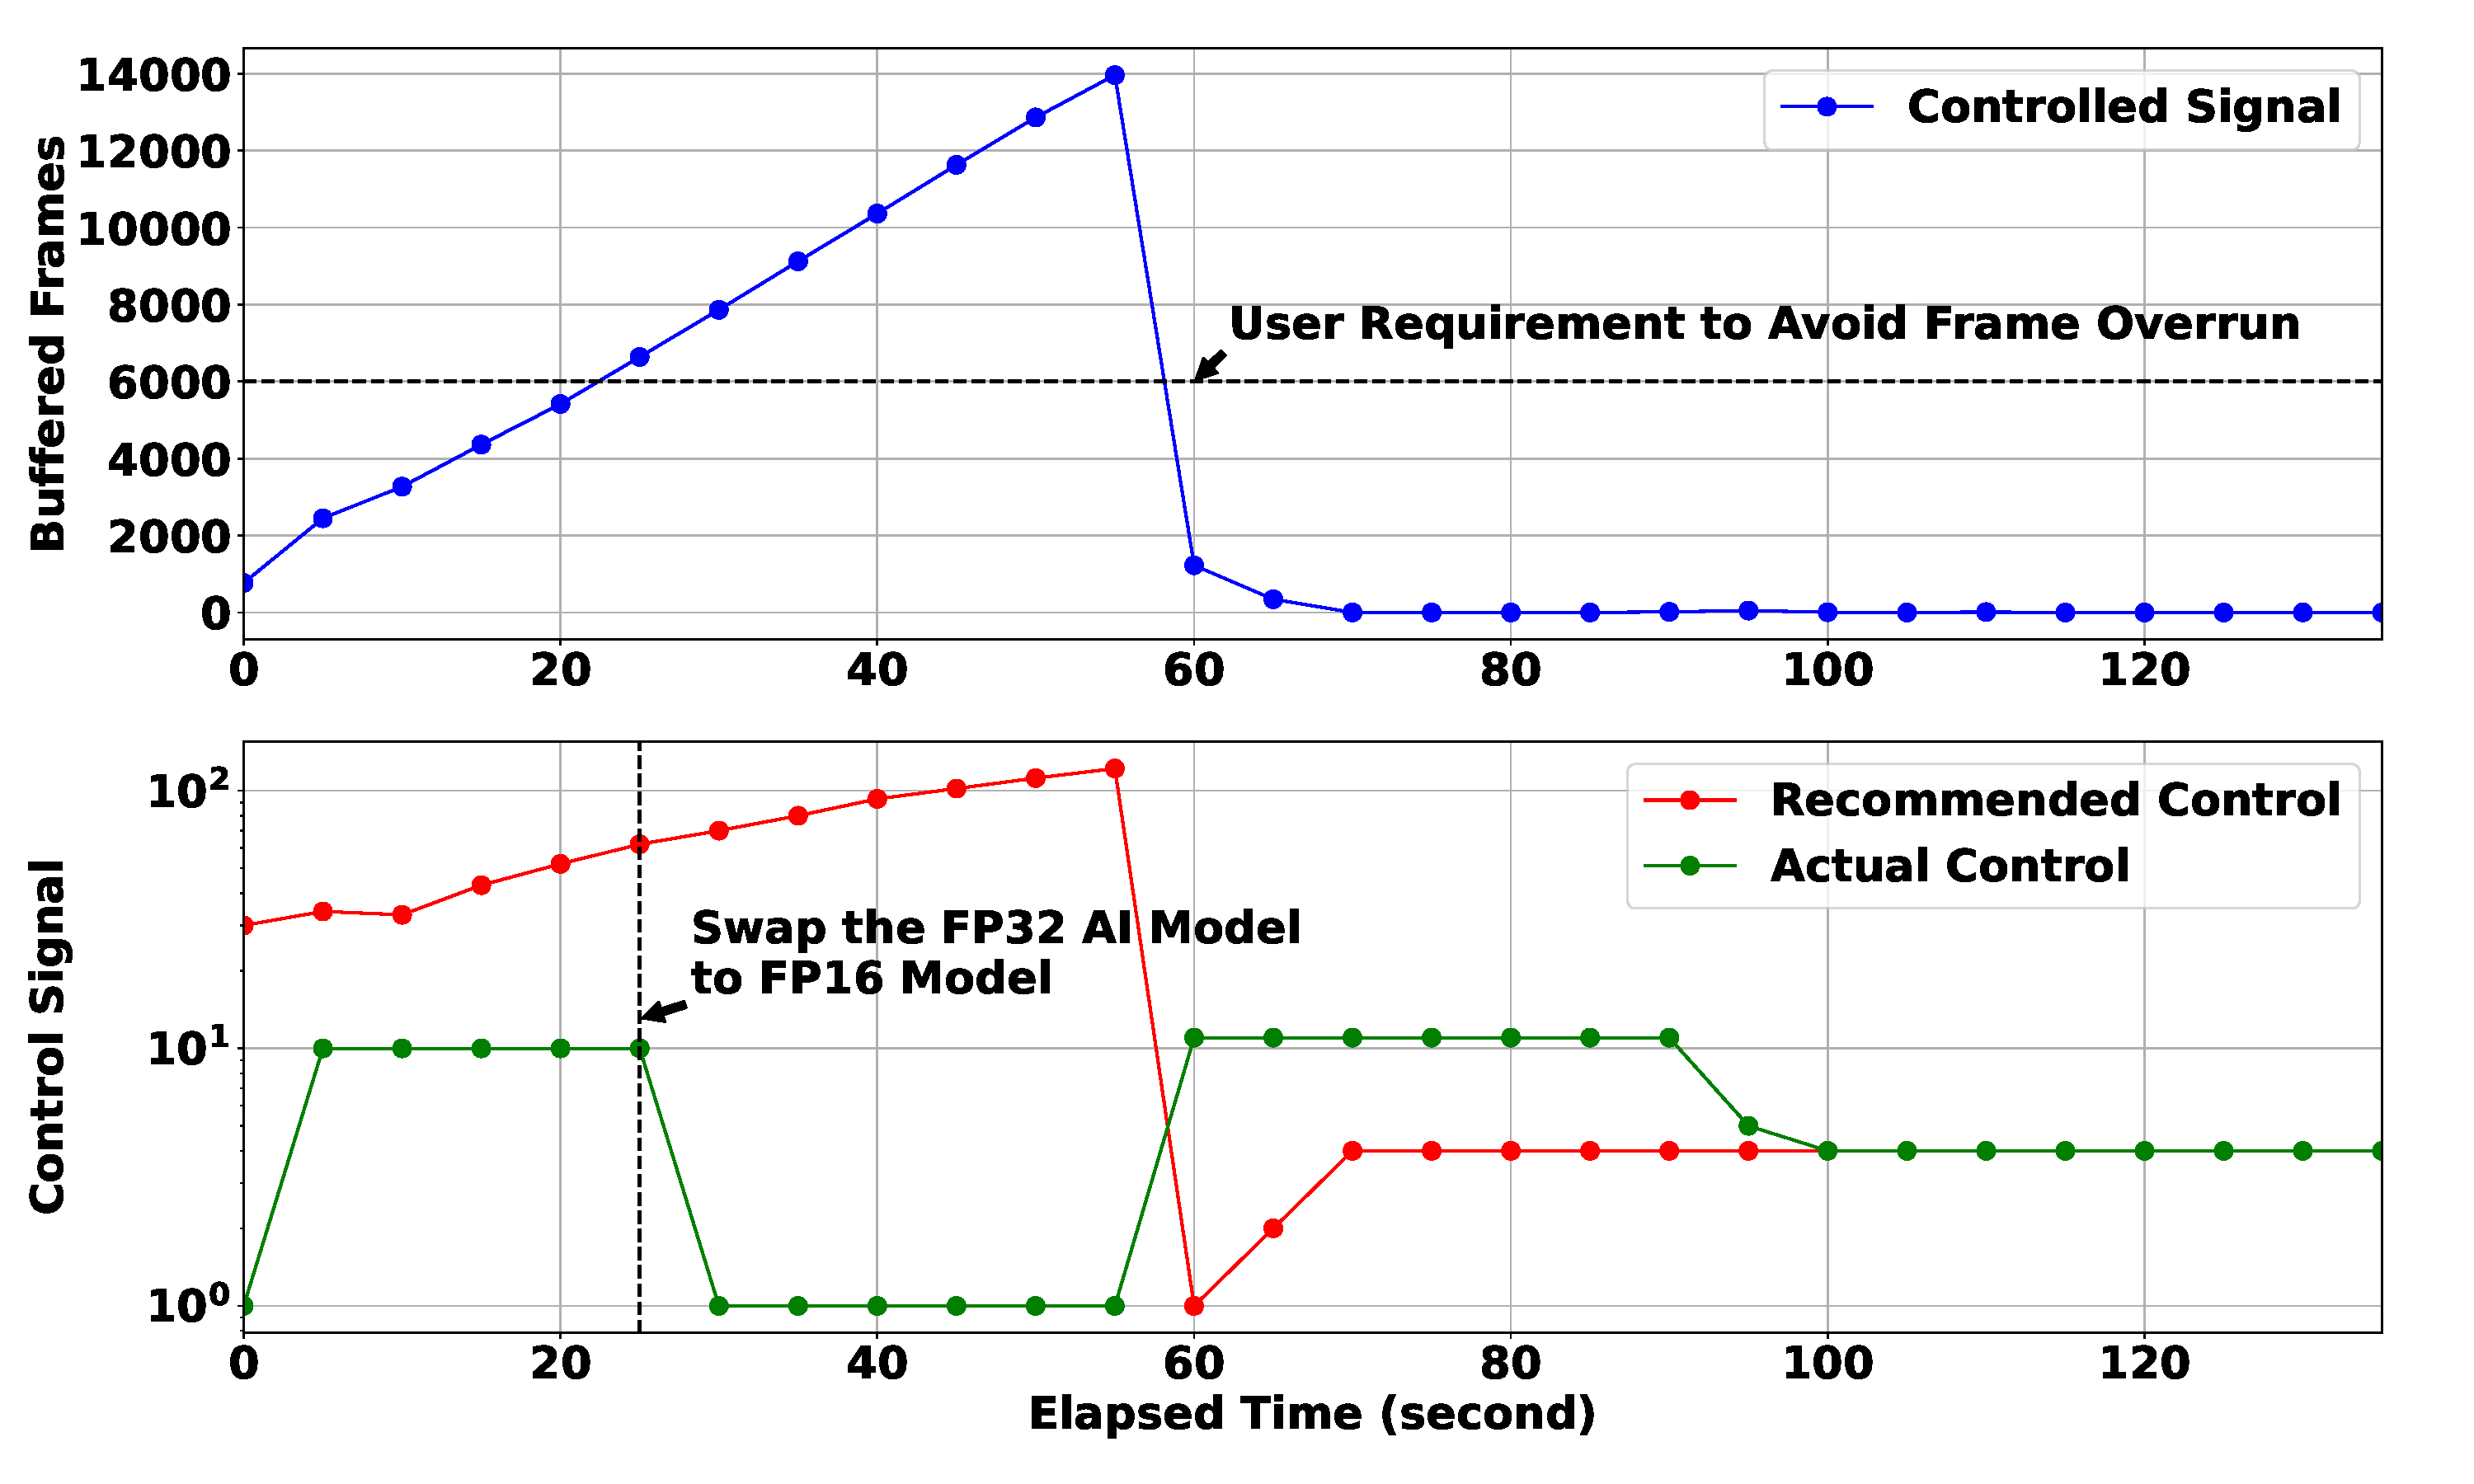
\includegraphics[width=\linewidth]{figures/adaptive_control.pdf}
  \caption{Demonstration of an adaptive PD controller, with $K_p = 0.5$ and $K_d = 1$. Per user requirement, the controller swapped the AI model to a smaller one to handle the incoming frame rate that overran the buffer.}
  \label{fig:adaptive-control-result}
\end{figure}

In this experiment, we demonstrate how an adaptive controller can be applied to overcome frame overrun. The PtychoNN AI model is prepared in single-precision floating point (FP32) and half-precision (FP16) after quantization. The reduced precision slightly degrades the AI performance but gains computing efficiency, for example, memory reduction and faster floating-point calculation. We set the experiment with a 400-FPS input stream to make the buffer overrun by incoming frames when using the FP32 model within the provided computing node. Then, we simulate a buffer overrun threshold set by a user, triggering a switch to the FP16 model.

Figure~\ref{fig:adaptive-control-result} showcases the control and performance of this setup. Starting with the FP32 model results in a buffer quickly filling with unprocessed frames. Once the controller detects that the buffered frames signal exceeds the set threshold, FP32 model containers are shutdown and swapped with the FP16 model ones. Control resumes after the transition, this time with reasonable performance, as the FP16 models can handle the incoming frame rate (as they process frames much faster than the FP32 model, even with a fewer number of container instances). Note that due to implementation limitations, frames already sent to a consumer are lost in the model transition process, resulting in a sharp drop in buffered frames. An application, or a streaming data pipeline infrastructure capable of keeping track of frames would prevent this, and require more control after the transition to quickly drain buffers.

\subsection{Discussion}

\begin{figure}[!tb]
  \centering
  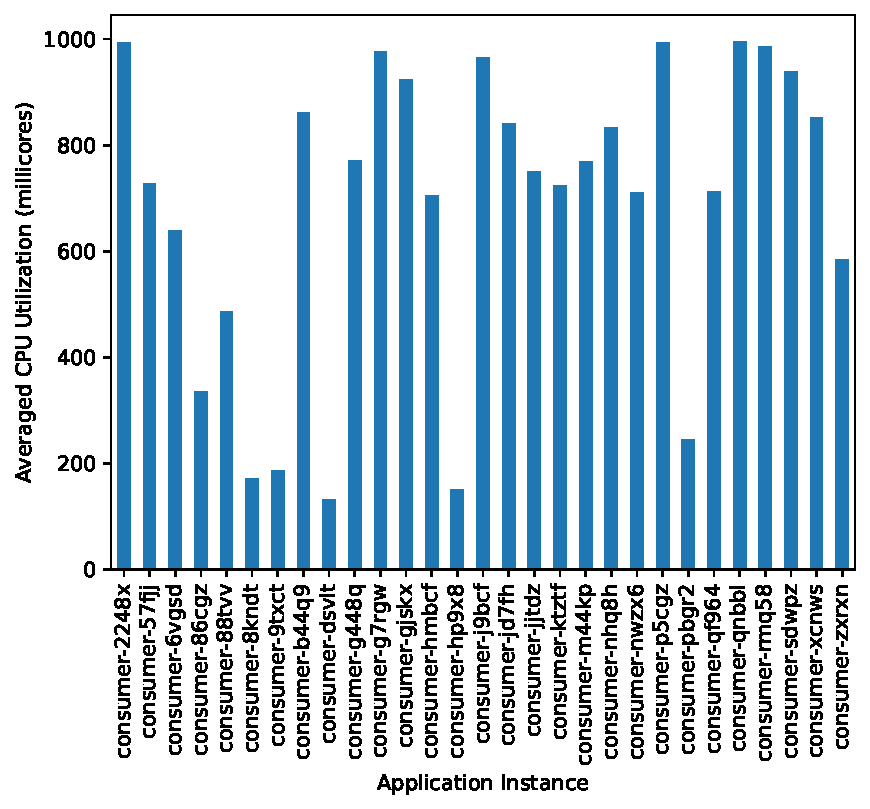
\includegraphics[width=\linewidth]{figures/cpu_utilization.pdf}
  \caption{Averaged CPU utilization per application instance. Note that 2 of the 31 instances were not measured because they were terminated too early by the controller.}
  \label{fig:cpuutil}
\end{figure}

\noindent\textbf{Resource Optimization} As shown in Fig.~\ref{fig:control-result}, the controller in the first experiment (see the subsection~\ref{subsec:first-experiment}) spawned 31 application instances in total, which consumed approximately 20 CPU cores and 23 GB of memory to handle the 1,000-FPS data stream. Each instance was allocated 1 CPU core but used different amounts over the experiment (see Fig.~\ref{fig:cpuutil}) because they were spawned at different times and the total X-ray images to process varied over time.

Edge resources are often limited, for example by the physical space available near
the experiment. In our current use case at the APS, this could lead to
multiple tenants (experiments) sharing edge resources. In such a setup and with such a dynamic behavior for each scientific workflow, finer-grained control of resource allocation would be desired, to ensure performance and fairness to each user.

\noindent\textbf{Model Size and Quantization} Model selection is one of the main factors in determining where the model runs in the heterogeneous edge-to-HPC continuum and what precision the selection offers. Smaller models process data much faster and run on less performant computing nodes. If a scientific experiment is robust to data quality reduction, model selection as a control action could provide more flexibility in the design and efficient use of AI@Edge systems.

\noindent\textbf{Container Run Time and AI Inference-as-a-Service} The application instances were a container run by Kubernetes. Each instance loaded the same model and dependent libraries within the container for AI inference. Although the programming model of the proposed framework is simple and easy to use, the initialization of an instance in the Kubernetes container run time took at least several seconds on a server-rack computer. In order to eliminate the duplicated library loading and react to rapid deployment and control of application instances, efficient programming models such as Nvidia Triton inference-as-a-service~\cite{savard2024optimizing} can be introduced in the framework. Similarly, enabling adaptation at each step of this scientific pipeline (data collection, preprocessing, inference) or our more developed use case (feature extraction, control, fine-tuning) would also provide opportunities for further performance improvements. We refer in particular to infrastructure stages for which hardware resources can be changed at run time (moldable jobs, heartbeat scheduling~\cite{acar2018heartbeat}).

% This is to reflect the reviewers' comments: 
% - It might perhaps be helpful to motivate how Charon can be used/what will need to be modified in other Edge-to-HPC use-cases (outside of APS). There will likely be few similarities and/or major differences. Identifying such similarities and outlining differences which might help broaden Charon's value more broadly.
% - Only one use case is presented. It would be helpful to discuss how common this specific scenario is or explore additional scenarios to illustrate broader applicability.
\subsection{Toward Broader Edge-to-HPC Applications}

\begin{figure}[!tb]
  \centering
  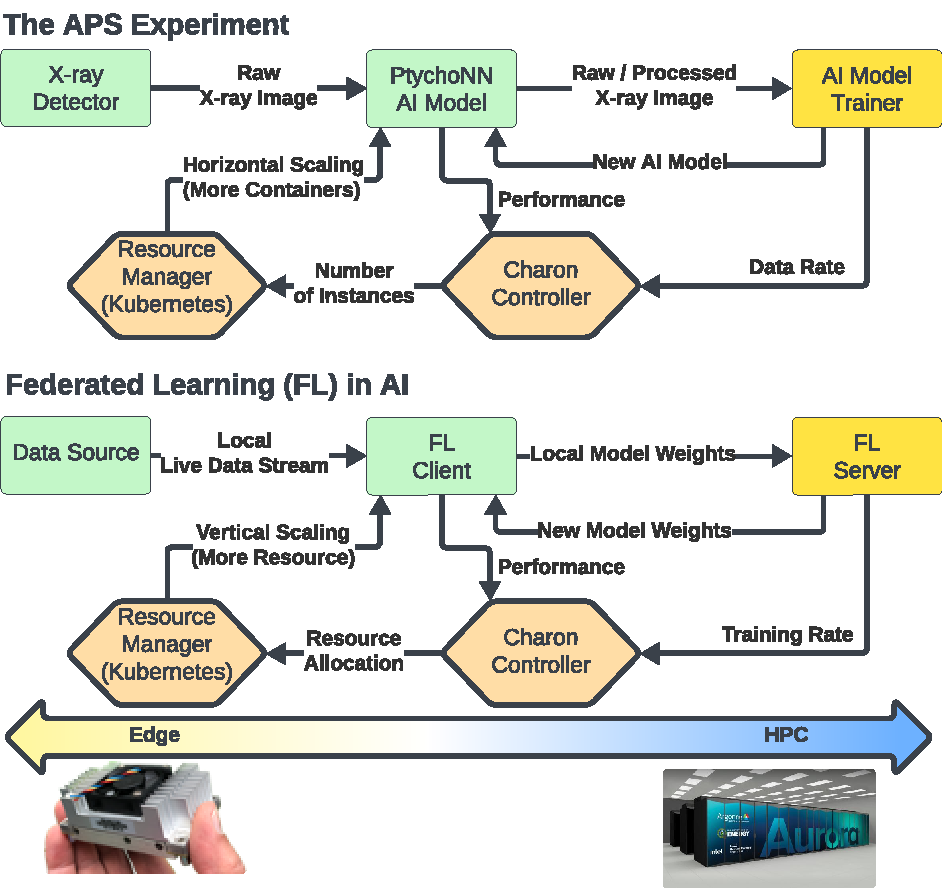
\includegraphics[width=\linewidth]{figures/usecases.pdf}
  \caption{Use cases in the Charon framework. The Charon controller drives computation at the edge while communicating with the HPC application for the holistic control in edge-to-HPC.}
  \label{fig:other-usecases}
\end{figure}

Although the work in this paper targets the APS use case, introduced in Section \ref{sec:usecase}, for real-time monitoring and control, the proposed framework and software stack bring fundamentals to support other edge-to-HPC applications. Figure \ref{fig:other-usecases} illustrates dataflow of the APS use case and the same for another use case, federated learning in edge-to-HPC. The Charon controller, the key fundamental, manages resources under local constraints and accepts inputs from both the edge and counter-part HPC applications. In the APS use case, the controller horizontally scales the AI application by sensing the application throughput. The AI trainer in HPC may set a specific data rate at which the trainer receives data from the edge to train a new model. Similarly, the federated learning (FL) client trains its local model with live data, while the FL server requests the local model weights from the client. The controller in this use case allocates more resources to the client if the server needs more training weights. This closed control loop allows many edge-to-HPC applications to manage their edge application at the high level in real time.

However, there are challenges in applying the proposed framework to potential edge-to-HPC applications. For example, the framework requires a communication channel to the applications with a descriptive language for the Charon controller to understand user requirements. Moreover, in an open network setup where edge nodes go online and offline and move their geo-location, the entire workflow should keep track of node availability to inject proper control inputs to the Charon controller in the node. Those challenges are left to the implementation to address.

% NOTE: due to the deadline we can't deliver this. But, we may be able to do in the camera ready version.
%\textcolor{red}{TODO: Can we do another experiment where the model's size changes in FP32 and FP16? Do we believe that this will make a difference in the throughput?}

% \textcolor{blue}{Reviewer 2: The experimental setup as well as the implementation plan sound reasonable. However, one thing I would have liked to see is to have some microbenchmark-style feasibility tests. Some examples are: - how long would it take to optimize the resource allocations?
% - whether Waggle nodes are capable of dealing with reconfiguration of the model?
% - what are the model sizes that can be accommodated?
% - how many multiple tenants can be supported simultaneously?}

% \textcolor{blue}{(Response: we described that the convergence time varies from the control parameters. )}

% To be filled. We should add ARgo / Waggle scheduler, Kubernetes scheduler, and other related works.

% We propose to build on previous pilot experiments between the Mathematics and Computer Science  Division and APS to construct an end-to-end prototype capable of operating at the APS upgraded data rates to provide fast, AI-driven, experimental steering that links parallel edge computing resources to Aurora for HPC-assisted AI inference at the edge. 
%
%We will extend and generalize these pilot experiments into a complete workflow, with advanced autotuning of low-level resource management to maximize
%the use of limited edge devices.
%
% We will explore the design space of system software to connect and adapt resource-constrained AI@Edge workloads to HPC. We will investigate how resource constraints on edge devices can be alleviated by dynamically adapting the edge environment, arbitrating resources to ensure the necessary performance for experiment-critical applications while enabling additional uses for the edge. We will explore how system software can help design AI@Edge applications that leverage HPC platforms to tune their models and redeploy improved models on the fly.

% Following this approach, we will research and demonstrate an end-to-end software infrastructure that enables efficient, end-to-end data extraction, reconfiguration of the AI model at run time, and control of experiments as they proceed---a first step towards building a “self-driving laboratory.”







% We envision the design of an end-to-end reconfigurable AI@Edge workflow as a system software and resource management problem: a low-level infrastructure must be provided to monitor the performance requirements of each component of the workflow running at the edge and ensure that dynamic factors such as related to data services or changes in workloads do not interfere with individual experiments. As the AI workloads themselves, as well as the data services dealing with data transfer between  edge and HPC resources, are use-case specific, this low-level infrastructure must be flexible. Both its mechanisms (what is being monitored, what actions can be taken) and its policies (e.g., how to search for better configurations) should be applicable across a wide range of experiments.

% \paragraph{Unknowns:}

% Our investigation will revolve around several key unknowns. \textbf{Signals and Controls:} what can  middleware for edge-level resource arbitration measure about the system and the application? what can be used as arbitration mechanisms? \textbf{Flexibility:} different instruments have different needs at the edge, including variability in hardware; how flexible/portable can resource arbitration policies be to support the widest range of configurations? \textbf{Stability:} how strict are resource requirements for instrument control applications? what level of noise can be tolerated? what are the constrains to reconfiguring an AI model on the fly without disrupting a given experiment?

%\noindent
%In order to realize this vision, we propose a limited-scope research expedition using existing research facilities and software to
%prototype such computing continuum middleware. Using well identified use cases from Argonne, we will demonstrate that resource
%management for AI@Edge can bring value to user facilities.